\chapter{Fonaments}

Es tracten en aquest cap\'{\i}tol q\"{u}estions b\`{a}siques
d'electrot\`{e}cnia, com ara teoremes, definicions i relacions.

\section{Teoremes d'electrot\`{e}cnia}\label{sec:teoremes}

\subsection{\texorpdfstring{Teorema de Th\'{e}venin--Norton}{Teorema de
            Th\'{e}venin-Norton}}\label{sec:T_N}

\index{teorema!de Th\'{e}venin}El teorema de Th\'{e}venin ens permet
substituir una xarxa complexa formada per elements lineals, per un
circuit equivalent format per una font de tensi\'{o} $\cmplx{E}\ped{Th}$
en s\`{e}rie amb una imped\`{a}ncia $\cmplx{Z}\ped{Th}$.

Atenent a la Figura \vref{pic:Thevenin}, si coneixem la tensi\'{o} en
buit $\cmplx{U}\ped{o}$ entre dos nusos $\alphaup$ i $\betaup$ d'una
xarxa, i la imped\`{a}ncia $\cmplx{Z}_{\alphaup\betaup}$ d'aquesta xarxa
vista des d'aquests dos nusos, podem obtenir els valors del circuit
Th\'{e}venin equivalent entre aquests dos nusos, a partir de les
relacions seg\"{u}ents:\index{ETh@$E\ped{Th}$}\index{ZTh@$Z\ped{Th}$}
\begin{equation}
   \cmplx{E}\ped{Th} = \cmplx{U}\ped{o} \qquad\qquad  \cmplx{Z}\ped{Th} = \cmplx{Z}_{\alphaup\betaup}
\end{equation}

D'aquesta manera, la connexi\'{o} d'aquesta xarxa a trav\'{e}s dels nusos
$\alphaup$ i $\betaup$ a una c\`{a}rrega qualsevol $\cmplx{Z}\ped{Q}$, \'{e}s
equivalent pel que fa a aquesta c\`{a}rrega, a connectar el circuit
equivalent Th\'{e}venin a la c\`{a}rrega.
\begin{figure}[htb]
\centering
    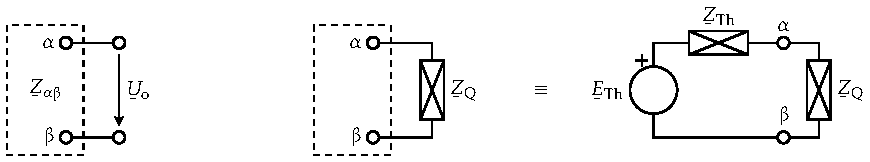
\includegraphics{Imatges/Cap-Fonaments-Thevenin.pdf}
\caption{Teorema de Th\'{e}venin} \label{pic:Thevenin}
\end{figure}

\index{teorema!de Norton}El teorema de Norton ens permet substituir
una xarxa complexa formada per elements lineals, per un circuit
equivalent format per una font de corrent $\cmplx{J}\ped{No}$ en
para{\l.l}el amb una admit\`{a}ncia $\cmplx{Y}\ped{No}$.

Atenent a la Figura \vref{pic:Norton}, si coneixem el corrent de
curt circuit $\cmplx{I}\ped{cc}$ entre dos nusos $\alphaup$ i $\betaup$
d'una xarxa, i l'admit\`{a}ncia $\cmplx{Y}_{\alphaup\betaup}$ d'aquesta
xarxa vista des d'aquests dos nusos, podem obtenir els valors del
circuit Norton equivalent entre aquests dos nusos, a partir de les
relacions seg\"{u}ents:\index{JNo@$J\ped{No}$}\index{YNo@$Y\ped{No}$}
\begin{equation}
   \cmplx{J}\ped{No} = \cmplx{I}\ped{cc} \qquad\qquad \cmplx{Y}\ped{No} = \cmplx{Y}_{\alphaup\betaup}
\end{equation}

D'aquesta manera, la connexi\'{o} d'aquesta xarxa a trav\'{e}s dels nusos
$\alphaup$ i $\betaup$ a una c\`{a}rrega qualsevol $\cmplx{Z}\ped{Q}$, \'{e}s
equivalent pel que fa a aquesta c\`{a}rrega, a connectar el circuit
equivalent Norton a la c\`{a}rrega.
\begin{figure}[h]
\centering
    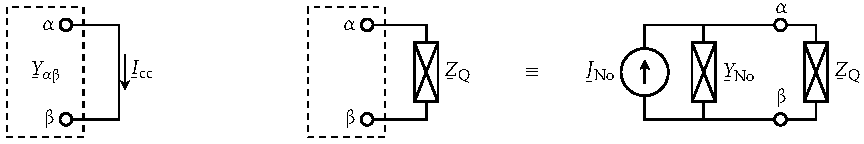
\includegraphics{Imatges/Cap-Fonaments-Norton.pdf}
\caption{Teorema de Norton} \label{pic:Norton}
\end{figure}

Els circuits Th\'{e}venin i Norton d'una xarxa s\'{o}n equivalents entre si.
Els par\`{a}metres que defineixen aquests circuits guarden les relacions
seg\"{u}ents:
\begin{equation}\label{eq:Thevenin-Norton}
   \cmplx{E}\ped{Th} = \frac{\cmplx{J}\ped{No}}{\cmplx{Y}\ped{No}} \qquad\qquad
   \cmplx{J}\ped{No} = \frac{\cmplx{E}\ped{Th}}{\cmplx{Z}\ped{Th}} \qquad\qquad
    \cmplx{Z}\ped{Th} = \frac{1}{\cmplx{Y}\ped{No}}
\end{equation}

Els valors $\cmplx{Z}\ped{Th}$ i  $\cmplx{Y}\ped{No}$ es poden
obtenir substituint en la xarxa  les fonts de tensi\'{o}  per curt
circuits, i les fonts de corrent per circuits oberts, i calculant
aleshores la imped\`{a}ncia o admit\`{a}ncia equivalent\footnote{El c\`{a}lcul sistem\`{a}tic de $\cmplx{Z}\ped{Th}$ i  $\cmplx{Y}\ped{No}$ en una xarxa qualsevol, s'exposa en la secci\'{o} \ref{sec:xarxes_Zth}}.

\subsection{Teorema de Millman}

\index{teorema!de Millman}Atenent a la Figura \vref{pic:Millman}, el teorema
de Millman ens permet
obtenir la tensi\'{o} de l'extrem com\'{u} $\nuup$ de diverses imped\`{a}ncies respecte d'un punt
qualsevol $\alphaup$, a partir de les tensions dels altres extrems de les imped\`{a}ncies respecte
 del mateix punt $\alphaup$.

\begin{figure}[htb]
%\vspace{0.3cm}
\hfill
\begin{minipage}[b]{7cm}
    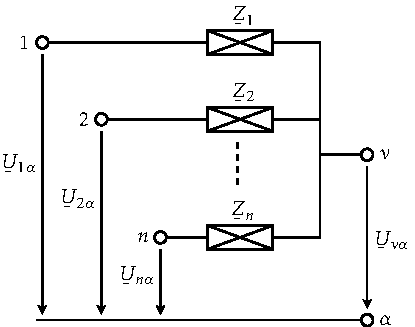
\includegraphics{Imatges/Cap-Fonaments-Millman.pdf}
    \caption{Teorema de Millman} \label{pic:Millman}
\end{minipage}
\hfill
\begin{minipage}[b][4.5cm][t]{6cm}
    \begin{equation}
        \cmplx{U}_{\nuup\alphaup} = \frac{\displaystyle\sum_{k=1}^n \dfrac{\cmplx{U}_{k\alphaup}}{\cmplx{Z}_k}} {\displaystyle\sum_{k=1}^n \dfrac{1}{\cmplx{Z}_k}}
    \end{equation}
\end{minipage}
\end{figure}

\begin{exemple}
A partir de la figura seg\"{u}ent, es tracta de determinar els circuits
Th\'{e}venin i Norton equivalents del circuit format per les tres
bateries i les seves resist\`{e}ncies, i calcular la tensi\'{o} i la
intensitat que existirien en una resist\`{e}ncia de c\`{a}rrega
$R\ped{Q}=50\unit{\ohm}$, que es connect\'{e}s entre els punts $\alphaup$
i $\nuup$.

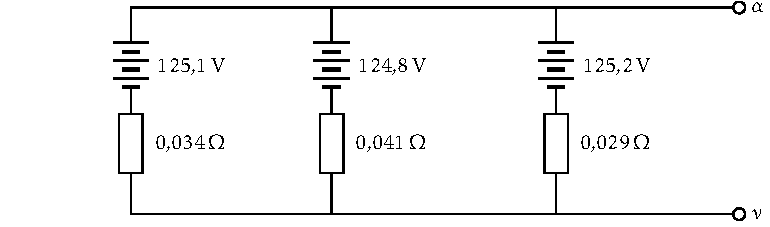
\includegraphics{Imatges/Cap-Fonaments-Millman-Exemple.pdf}

La imped\`{a}ncia Th\'{e}venin equivalent es calcula, tal com s'ha dit en la Secci\'{o} \ref{sec:T_N},
substituint en el circuit totes les fonts de tensi\'{o} per curt circuits, aix\'{\i} doncs, ens
queden tres resist\`{e}ncies en para{\l.l}el entre $\alphaup$ i $\nuup$:
\[
Z\ped{Th} = R_{\alphaup\nuup} =\frac{1}{\dfrac{1}{0{,}034\unit{\ohm}} +
\dfrac{1}{0{,}041\unit{\ohm}} + \dfrac{1}{0{,}029\unit{\ohm}}} =
0{,}01133\unit{\ohm}
\]

Per calcular la font de tensi\'{o} Th\'{e}venin equivalent, utilitzarem el
teorema de Millman. Si es compara aquest circuit amb el de la Figura
\vref{pic:Millman}, veiem que els punts $\alphaup$ i $\nuup$ dels dos
circuits s\'{o}n equivalents, \'{e}s a dir, $\nuup$ \'{e}s el punt com\'{u} de les
imped\`{a}ncies, i $\alphaup$ \'{e}s el punt de refer\`{e}ncia dels altres extrems
de les imped\`{a}ncies, respecte del qual les tensions s\'{o}n conegudes
(tensions de les bateries). Aix\'{\i} doncs tenim:
\[
U_{\nuup\alphaup} = \frac{\dfrac{-125{,}1\unit{V}}{0{,}034\unit{\ohm}} +
\dfrac{-124{,}8\unit{V}}{0{,}041\unit{\ohm}} +
\dfrac{-125{,}2\unit{V}}{0{,}029\unit{\ohm}}}{\dfrac{1}{0{,}034\unit{\ohm}}
+ \dfrac{1}{0{,}041\unit{\ohm}} + \dfrac{1}{0{,}029\unit{\ohm}}} =
-125{,}0562\unit{V}
\]

La font de tensi\'{o}  Th\'{e}venin equivalent entre $\alphaup$ i $\nuup$ \'{e}s per
tant:
\[
E\ped{Th} = U_{\alphaup\nuup} = 125{,}0562\unit{V}
\]

Calculem a continuaci\'{o} l'admit\`{a}ncia i la font de corrent  Norton equivalents, utilitzant
l'equaci\'{o} \eqref{eq:Thevenin-Norton}:
\begin{align*}
    Y\ped{No} &= \frac{1}{Z\ped{Th}} = \frac{1}{0{,}01133\unit{\ohm}} = 82{,}2613\unit{S}
    \\[2ex]
    J\ped{No} &= \frac{E\ped{Th}}{Z\ped{Th}} =
    \frac{125{,}0562\unit{V}}{0{,}01133\unit{\ohm}}= 11037{,}6150\unit{A}
\end{align*}

Tal com s'ha dit en la Secci\'{o} \ref{sec:T_N}, J\ped{No} \'{e}s igual a la
intensitat de curt circuit entre els punts $\alphaup$ i $\nuup$.

Finalment, ja podem calcular el corrent $I\ped{Q}$ i la tensi\'{o} $U\ped{Q}$ en la
resist\`{e}ncia de c\`{a}rrega, utilitzant el circuit Th\'{e}venin equivalent calculat anteriorment:
\begin{align*}
    I\ped{Q} &= \frac{E\ped{Th}}{Z\ped{Th} + R\ped{Q}} = \frac{125{,}0562\unit{V}}
    {0{,}01133\unit{\ohm} + 50\unit{\ohm}} = 2{,}5001\unit{A} \\[2ex]
    U\ped{Q} &=  R\ped{Q} \,I\ped{Q} = 50\unit{\ohm} \cdot 2{,}5001\unit{A} =
    125{,}0050\unit{V}
\end{align*}
\end{exemple}


\subsection{Teorema de la superposici\'{o}}\index{teorema!de la
superposici\'{o}}

Si tenim un circuit lineal on hi ha diverses fonts de tensi\'{o} i  de
corrent, les quals originen corrents i caigudes de tensi\'{o} en els
components del circuit, el teorema de la superposici\'{o} ens diu que
podem calcular aquests corrents i caigudes de tensi\'{o}, resolent els
circuits que resulten de tenir en compte  nom\'{e}s una font de tensi\'{o} o
de corrent a l'hora, i sumant al final els valors parcials
obtinguts.

En cada pas on considerem nom\'{e}s una font de tensi\'{o} o de corrent, hem
d'eliminar la resta de fonts del circuit; per tal de fer-ho hem de
substituir la resta de fonts de tensi\'{o} per un curt circuit, i la
resta de fonts de corrent per un circuit obert.

Aquest teorema tamb\'{e} \'{e}s aplicable en el cas que tinguem nom\'{e}s una
font de tensi\'{o} o de corrent, que operi a m\'{e}s d'una freq\"{u}\`{e}ncia a
l'hora. En aquest cas es pot estudiar el circuit de forma
independent per a cadascuna de les freq\"{u}\`{e}ncies presents, i sumar al
final els valors parcials obtinguts.

\begin{exemple}
    Es tracta de trobar en el circuit seg\"{u}ent, el corrent $\cmplx{I}$ que circula
    pel condensador, utilitzant el teorema de la superposici\'{o}.
    \begin{figure}[htb]
        \centering
        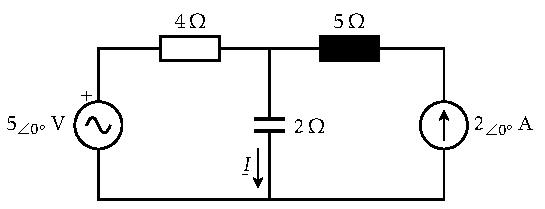
\includegraphics{Imatges/Cap-Fonaments-Exemple-Superposicio-1.pdf}
    \end{figure}

    Utilitzant el teorema de la superposici\'{o}, representem els dos
    circuits seg\"{u}ents a partir del circuit original. El circuit de
    l'esquerra nom\'{e}s t\'{e} la font de tensi\'{o}, amb la font de corrent
    substitu\"{\i}da per un circuit obert, i el circuit de
    la dreta nom\'{e}s t\'{e} la font de corrent, amb la font de tensi\'{o}
    substitu\"{\i}da per un curt circuit.
    \begin{figure}[htb]
        \centering
        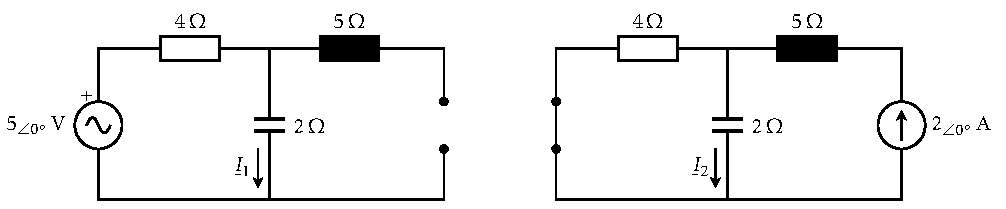
\includegraphics{Imatges/Cap-Fonaments-Exemple-Superposicio-2.pdf}
    \end{figure}

    Els corrents $\cmplx{I}_1$ i $\cmplx{I}_2$ que circulen pel condensador valen:
    \[
        \cmplx{I}_1 = \frac{5_{\angle 0\degree}\unit{V}}{(4-\ju
        2)\unit{\ohm}} = 1{,}118_{\angle
        26{,}57\degree}\unit{A} \qquad\qquad
        \cmplx{I}_2 = \frac{\dfrac{1}{\frac{1}{4\unit{\ohm}}+\frac{1}{-\ju 2\unit{\ohm}}}}
        {-\ju 2\unit{\ohm}} \, 2_{\angle 0\degree}\unit{A} = 1{,}789_{\angle
        26{,}57\degree}\unit{A}
    \]

    El corrent total $\cmplx{I}$ que circula pel condensador val:
    \[
        \cmplx{I}  = \cmplx{I}_1 + \cmplx{I}_2 = 1{,}118_{\angle
        26{,}57\degree}\unit{A} + 1{,}789_{\angle
        26{,}57\degree}\unit{A} =
        2{,}907_{\angle 26{,}57\degree}\unit{A}
    \]
\end{exemple}


\section{Components elementals d'un circuit
el\`{e}ctric}\label{sec:comp_elem}

Es presenten a continuaci\'{o} les lleis temporals que lliguen tensions,
corrents i pot\`{e}ncies, per a diversos components elementals d'un
circuit el\`{e}ctric. Es donen tamb\'{e} les relacions entre tensions i
corrents en el domini freq\"{u}encial (corrent altern sinuso\"{\i}dal, amb
$\omega=2\piup f$) i en el domini operacional (transformada de
Laplace).\index{transformada de Laplace}

Cal tenir en compte que les relacions que es donen, tan sols s\'{o}n
v\`{a}lides  quan es tenen en consideraci\'{o} els sentits assignats als
corrents i a les tensions en les figures corresponents.

\subsection{Resist\`{e}ncia} \index{resist\`{e}ncia}

\index{resist\`{e}ncia!llei temporal}Per a una resist\`{e}ncia $R$ (Figura
\vref{pic:resist}), la llei temporal entre la tensi\'{o} $u(t)$ i el
corrent $i(t)$, i la llei temporal de la pot\`{e}ncia $p(t)$ s\'{o}n:
\vspace{-0.5mm}
\begin{figure}[h!]
\hfill
\begin{minipage}[b]{5cm}
    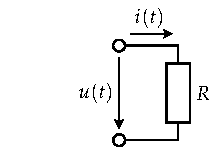
\includegraphics{Imatges/Cap-Fonaments-Resistencia.pdf}
\caption{Resist\`{e}ncia} \label{pic:resist}
\end{minipage}
\hfill
\begin{minipage}[b][3.25cm][t]{8cm}
   \begin{align}
      u(t) &= R i(t) \\  p(t) &= u(t) i(t) = R i^2(t) = \frac{u^2(t)}{R}
   \end{align}
\end{minipage}
\end{figure}

\index{resist\`{e}ncia!domini freq\"{u}encial}En el domini freq\"{u}encial, la relaci\'{o} entre
la tensi\'{o} $\cmplx{U}$ i el corrent $\cmplx{I}$, i la relaci\'{o} entre els arguments de
la tensi\'{o} $\varphi_{\cmplx{U}}$ i del corrent $\varphi_{\cmplx{I}}$ s\'{o}n:
\begin{align}
   \cmplx{U} &= R \cmplx{I} \\ \varphi_{\cmplx{U}} &= \varphi_{\cmplx{I}}
\end{align}

\index{resist\`{e}ncia!domini operacional} En el domini operacional, la relaci\'{o} entre la tensi\'{o} $U(s)$ i el corrent $I(s)$ \'{e}s:
\begin{equation}
   U(s) = R I(s)
\end{equation}

\subsection{Capacitat} \index{capacitat}

\index{capacitat!llei temporal}Per a una capacitat $C$ (Figura
\vref{pic:capacit}), les lleis temporals entre la tensi\'{o} $u(t)$ i el
corrent $i(t)$, i la llei temporal de la pot\`{e}ncia $p(t)$ s\'{o}n:
\vspace{-1.5mm}
\begin{figure}[h!]
\hfill
\begin{minipage}[b]{5cm}
    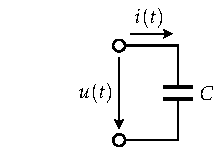
\includegraphics{Imatges/Cap-Fonaments-Capacitat.pdf}
\caption{Capacitat} \label{pic:capacit}
\end{minipage}
\hfill
\begin{minipage}[b][3.8cm][t]{8cm}
   \begin{align}
      u(t) &= u(t_0) + \frac{1}{C} \int_{t_0}^t i(t) \diff t \\
      i(t) &= C \deriv{u(t)}{t} \\
      p(t) &= u(t) i(t) = C u(t) \deriv{u(t)}{t}
   \end{align}
\end{minipage}
\end{figure}

\index{capacitat!domini freq\"{u}encial}En el domini freq\"{u}encial, la relaci\'{o} entre la tensi\'{o} $\cmplx{U}$ i el corrent $\cmplx{I}$, i la relaci\'{o} entre els arguments de la tensi\'{o} $\varphi_{\cmplx{U}}$ i del corrent $\varphi_{\cmplx{I}}$ s\'{o}n:
\begin{align}
   \cmplx{U} &= -\ju \frac{1}{\omega C} \cmplx{I} \\
   \varphi_{\cmplx{U}} &= \varphi_{\cmplx{I}} - \frac{\piup}{2}
\end{align}

\index{capacitat!domini operacional}En el domini operacional, la relaci\'{o} entre la tensi\'{o} $U(s)$ i el corrent $I(s)$ \'{e}s:
\begin{equation}
   U(s) = \frac{1}{s C} I(s) + \frac{u(t_0)}{s}
\end{equation}


\subsection{Induct\`{a}ncia} \index{induct\`{a}ncia}

\index{induct\`{a}ncia!llei temporal}Per a una induct\`{a}ncia $L$ (Figura \vref{pic:induct}),
les lleis temporals entre la tensi\'{o} $u(t)$ i el corrent $i(t)$, i la llei temporal
de la pot\`{e}ncia $p(t)$ s\'{o}n:
\begin{figure}[htb]
\hfill
\begin{minipage}[b]{5cm}
    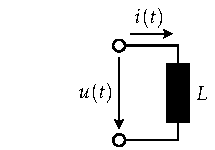
\includegraphics{Imatges/Cap-Fonaments-Inductancia.pdf}
\caption{Induct\`{a}ncia} \label{pic:induct}
\end{minipage}
\hfill
\begin{minipage}[b][3.8cm][t]{8cm}
   \begin{align}
      i(t) &= i(t_0) + \frac{1}{L} \int_{t_0}^t u(t) \diff t \\
      u(t) &= L \deriv{i(t)}{t} \\
      p(t) &= u(t) i(t) = L i(t) \deriv{i(t)}{t}
   \end{align}
\end{minipage}
\end{figure}

\index{induct\`{a}ncia!domini freq\"{u}encial}En el domini freq\"{u}encial, la relaci\'{o} entre la tensi\'{o} $\cmplx{U}$ i el corrent $\cmplx{I}$, i la relaci\'{o} entre els arguments de la tensi\'{o} $\varphi_{\cmplx{U}}$ i del corrent $\varphi_{\cmplx{I}}$ s\'{o}n:
\begin{align}
   \cmplx{U} &= \ju \omega L \cmplx{I} \\
   \varphi_{\cmplx{U}} &= \varphi_{\cmplx{I}} + \frac{\piup}{2}
\end{align}

\index{induct\`{a}ncia!domini operacional} En el domini operacional, la relaci\'{o} entre la tensi\'{o} $U(s)$ i el corrent $I(s)$ \'{e}s:
\begin{equation}
   U(s) = s L I(s) - L i(t_0)
\end{equation}


\subsection{Acoblament magn\`{e}tic} \index{acoblament magn\`{e}tic}

\index{acoblament magn\`{e}tic!llei temporal}Per a un acoblament magn\`{e}tic $M$ entre dues
induct\`{a}ncies $L_1$ i $L_2$ (Figura \vref{pic:acobl}), les lleis temporals entre les
tensions $u_1(t)$ i $u_2(t)$ i els corrents $i_1(t)$ i $i_2(t)$,  i la llei temporal
de la pot\`{e}ncia $p(t)$ s\'{o}n: \pagebreak
\begin{figure}[h!]
\hfill
\begin{minipage}[b]{6cm}
   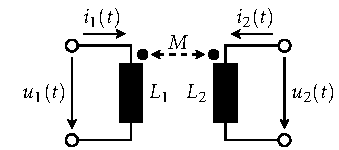
\includegraphics{Imatges/Cap-Fonaments-Acobl-Magnetic.pdf}
   \caption{Acoblament magn\`{e}tic} \label{pic:acobl}
\end{minipage}
\hfill
\begin{minipage}[b][3.8cm][t]{10cm}
   \begin{align}
      u_1(t) &= L_1 \deriv{i_1(t)}{t} + M \deriv{i_2(t)}{t} \\
      u_2(t) &= L_2 \deriv{i_2(t)}{t} + M \deriv{i_1(t)}{t} \\
      p(t) &= \frac{\diff}{\diff t} \left[ \frac{1}{2} L_1 i_1^2(t) + \frac{1}{2} L_2 i_2^2(t) +
      M i_1(t) i_2(t) \right]
   \end{align}
\end{minipage}
\end{figure}

\index{acoblament magn\`{e}tic!domini freq\"{u}encial}En el domini freq\"{u}encial, les relacions entre les tensions $\cmplx{U}_1$ i $\cmplx{U}_2$ i els corrents $\cmplx{I}_1$ i $\cmplx{I}_2$ s\'{o}n:
\begin{align}
   \cmplx{U}_1 &= \ju \omega L_1 \cmplx{I}_1 + \ju \omega M \cmplx{I}_2 \\
   \cmplx{U}_2 &= \ju \omega L_2 \cmplx{I}_2 + \ju \omega M \cmplx{I}_1
\end{align}

\index{acoblament magn\`{e}tic!domini operacional}En el domini operacional, les relacions entre les tensions $U_1(s)$  i $U_2(s)$ i els corrents $I_1(s)$ i $I_2(s)$ s\'{o}n:
\begin{align}
   U_1(s) &= s L_1 I_1(s) - L_1 i_1(t_0) + s M I_2(s) - M i_2(t_0) \\
   U_2(s) &= s L_2 I_2(s) - L_2 i_2(t_0) + s M I_1(s) - M i_1(t_0)
\end{align}

\subsection{Transformador ideal} \index{transformador ideal}

\index{transformador ideal!llei temporal}Per a un transformador
ideal de relaci\'{o} $m\!:\!1$ (Figura \vref{pic:transf}), la llei temporal
entre les tensions de primari $u_1(t)$ i de secundari $u_2(t)$, la
llei temporal entre els corrents de primari $i_1(t)$ i de secundari
$i_2(t)$, i la llei temporal de la pot\`{e}ncia $p(t)$ s\'{o}n:
\begin{figure}[htb]
\hfill
\begin{minipage}[b]{6cm}
    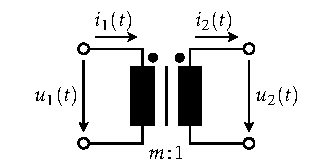
\includegraphics{Imatges/Cap-Fonaments-Trafo-Ideal.pdf}
\caption{Transformador ideal} \label{pic:transf}
\end{minipage}
\hfill
\begin{minipage}[b][3.7cm][t]{10cm}
   \begin{align}
      \frac{u_1(t)}{u_2(t)} &= m  \\
      \frac{i_2(t)}{i_1(t)} &= m \\
      p(t) &= u_1(t) i_1(t) - u_2(t) i_2(t) = 0
   \end{align}
\end{minipage}
\end{figure}

\index{transformador ideal!domini freq\"{u}encial} En el domini
freq\"{u}encial, la relaci\'{o} entre les tensions de primari $\cmplx{U}_1$
i de secundari $\cmplx{U}_2$, la relaci\'{o} entre els corrents de
primari $\cmplx{I}_1$ i de secundari $\cmplx{I}_2$, la relaci\'{o} entre
els arguments de les tensions de primari $\varphi_{\cmplx{U}_1}$ i
de secundari $\varphi_{\cmplx{U}_2}$, i  la relaci\'{o} entre els
arguments dels corrents de primari $\varphi_{\cmplx{I}_1}$ i de
secundari $\varphi_{\cmplx{I}_2}$ s\'{o}n:
\begin{align}
   \frac{\cmplx{U}_1}{\cmplx{U}_2} &= m  \\
   \frac{\cmplx{I}_2}{\cmplx{I}_1} &= m \\
   \varphi_{\cmplx{U}_1} &= \varphi_{\cmplx{U}_2} \\
   \varphi_{\cmplx{I}_1} &= \varphi_{\cmplx{I}_2}
\end{align}

\index{transformador ideal!domini operacional} En el domini operacional, la relaci\'{o} entre les tensions de primari $U_1(s)$ i de secundari $U_2(s)$,  i la relaci\'{o} entre els corrents de primari $I_1(s)$ i de secundari $I_2(s)$ s\'{o}n:
\begin{align}
   \frac{U_1(s)}{U_2(s)} &= m  \\
   \frac{I_2(s)}{I_1(s)} &= m
\end{align}

\subsection{Bateria} \index{bateria}

\index{bateria!llei temporal}Per a una bateria $U\ped{bat}$ (Figura
\vref{pic:bat}), la llei temporal de la tensi\'{o} $u(t)$ i de la
pot\`{e}ncia $p(t)$ que subministra \'{e}s:
\begin{figure}[h!]
\hfill
\begin{minipage}[b]{5cm}
    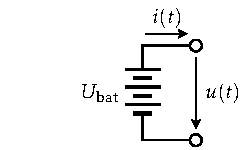
\includegraphics{Imatges/Cap-Fonaments-Bateria.pdf}
\caption{Bateria} \label{pic:bat}
\end{minipage}
\hfill
\begin{minipage}[b][3cm][t]{8cm}
   \begin{align}
      u(t) &= U\ped{bat} \\  p(t) &= U\ped{bat} i(t)
   \end{align}
\end{minipage}
\end{figure}

El corrent $i(t)$ que circular\`{a} per la bateria, vindr\`{a} determinat
pels elements que es connectin a aquesta bateria.

\index{bateria!domini operacional} En el domini operacional, la
tensi\'{o} $U(s)$ \'{e}s:
\begin{equation}
   U(s) = \frac{U\ped{bat}}{s}
\end{equation}

\section{Pot\`{e}ncia complexa}\label{sec:pot_complex} \index{pot\`{e}ncia complexa}

\subsection{Pot\`{e}ncia monof\`{a}sica} \index{pot\`{e}ncia complexa!monof\`{a}sica}

En la Figura \vref{pic:pot_comp_mono} es representa una c\`{a}rrega $\cmplx{Z}=R+\ju X$, la
qual absorbeix una pot\`{e}ncia complexa $\cmplx{S} = P + \ju Q$.

$R$ i $X$ s\'{o}n respectivament la part resistiva i la part reactiva
(inductiva o capacitiva) de la c\`{a}rrega, i $P$ i $Q$ s\'{o}n
respectivament la potencia activa i la potencia reactiva (inductiva
o capacitiva) absorbida per la c\`{a}rrega.

La pot\`{e}ncia activa absorbida per una c\`{a}rrega sempre \'{e}s positiva, en
canvi, la pot\`{e}ncia reactiva absorbida per una c\`{a}rrega pot ser
positiva o negativa, segons que predomini m\'{e}s la part inductiva o la
part capacitiva de la c\`{a}rrega respectivament.

\begin{figure}[htb]
\centering
    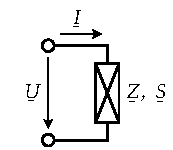
\includegraphics{Imatges/Cap-Fonaments-Potencia-Monof.pdf}
\caption{Pot\`{e}ncia complexa monof\`{a}sica} \label{pic:pot_comp_mono}
\end{figure}

L'angle $\varphiup$ entre els fasors $\cmplx{U}$ i $\cmplx{I}$ compleix la seg\"{u}ent relaci\'{o}:
\begin{equation}
   \tan\varphiup = \frac{X}{R} = \frac{Q}{P}
\end{equation}

\index{factor!de pot\`{e}ncia}A partir d'aquest angle $\varphiup$, es
defineix el factor de pot\`{e}ncia de la c\`{a}rrega:
\begin{equation}
   \text{Factor de pot\`{e}ncia} \equiv \cos\varphiup
\end{equation}

At\`{e}s que per a un angle qualsevol $\alphaup$ es compleix la igualtat
trigonom\`{e}trica: $\cos\alphaup = \cos(-\alphaup)$, quan es d\'{o}na el factor
de pot\`{e}ncia d'una c\`{a}rrega, cal especificar si \'{e}s inductiu ($Q>0,
\tan\varphiup>0$) o capacitiu ($Q<0, \tan\varphiup<0$); aix\`{o} es fa
afegint {"<}(i){">} o {"<}(c){">} respectivament al valor num\`{e}ric del factor
de pot\`{e}ncia, com per exemple: $\cos\varphiup=0,8$(i),
$\cos\varphiup=0,9$(c).

Les relacions que lliguen la pot\`{e}ncia complexa amb la tensi\'{o} i el corrent s\'{o}n:
\begin{align}
   \cmplx{S} &=  \cmplx{U} \,\cmplx{I}^* =
   |\cmplx{I}|^2 \,\cmplx{Z} = \frac{|\cmplx{U}|^2}{\cmplx{Z}^*} =
   P + \ju Q \label{eq:s_mono1}\\
   |\cmplx{S}| &= |\cmplx{U}| \,|\cmplx{I}| =
   |\cmplx{I}|^2 \,|\cmplx{Z}| = \frac{|\cmplx{U}|^2}{|\cmplx{Z}|} =
   \sqrt{P^2+Q^2} \\
   P &= \Re (\cmplx{U} \, \cmplx{I}^*) = |\cmplx{S}| \cos\varphiup =
   |\cmplx{U}|\, |\cmplx{I}| \cos\varphiup = |\cmplx{I}|^2 R =
   \frac{|\cmplx{U}|^2}{|\cmplx{Z}|^2}R\\
   Q &= \Im (\cmplx{U} \, \cmplx{I}^*) = |\cmplx{S}| \sin\varphiup =
   |\cmplx{U}| \,|\cmplx{I}|\sin\varphiup  = |\cmplx{I}|^2 X =
   \frac{|\cmplx{U}|^2}{|\cmplx{Z}|^2}X
\end{align}

\subsection{Pot\`{e}ncia trif\`{a}sica} \index{pot\`{e}ncia complexa!trif\`{a}sica}

En la Figura \vref{pic:pot_comp_trif} es representen dos sistemes
d'alimentaci\'{o} a c\`{a}rregues trif\`{a}siques; el de l'esquerra \'{e}s un
sistema de 4 fils (3 fases + neutre) i el de la dreta \'{e}s un sistema
de 3 fils (3 fases). En ambd\'{o}s casos es consideren tres c\`{a}rregues
$\cmplx{Z}_\alphaup = R_\alphaup + \ju X_\alphaup$, $\cmplx{Z}_\betaup=
R_\betaup + \ju X_\betaup$ i $\cmplx{Z}_\gammaup= R_\gammaup + \ju X_\gammaup$
connectades en estrella, les quals absorbeixen respectivament unes
pot\`{e}ncies complexes $\cmplx{S}_\alphaup= P_\alphaup + \ju Q_\alphaup$,
$\cmplx{S}_\betaup= P_\betaup + \ju Q_\betaup$ i $\cmplx{S}_\gammaup=
P_\gammaup + \ju Q_\gammaup$.

$R_\alphaup$, $R_\betaup$ i $R_\gammaup$, i $X_\alphaup$, $X_\betaup$ i
$X_\gammaup$ s\'{o}n respectivament les parts resistives i les parts
reactives (inductives o capacitives) de les c\`{a}rregues, i $P_\alphaup$,
$P_\betaup$ i $P_\gammaup$, i $Q_\alphaup$, $Q_\betaup$ i $Q_\gammaup$ s\'{o}n
respectivament les potencies actives i les potencies reactives
(inductives o capacitives) absorbides per les c\`{a}rregues.

El sistema d'alimentaci\'{o} de 3 fils, admet tamb\'{e} c\`{a}rregues
trif\`{a}siques connectades en triangle; en aquest cas nom\'{e}s cal dur a
terme la transformaci\'{o} a una connexi\'{o} en estrella (vegeu la Secci\'{o}
\ref{secc:d_y}), i per tant, la descripci\'{o} que segueix es pot
considerar del tot general.

\begin{figure}[h]
\centering
    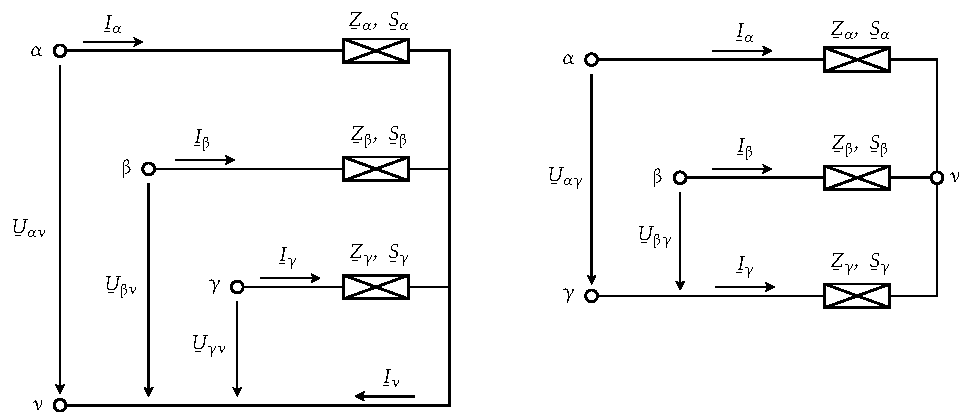
\includegraphics{Imatges/Cap-Fonaments-Potencia-Trif.pdf}
\caption{Pot\`{e}ncia complexa trif\`{a}sica. Sistemes de 4 fils i 3 fils
respectivament.} \label{pic:pot_comp_trif}
\end{figure}

En el cas m\'{e}s general, on la c\`{a}rrega trif\`{a}sica \'{e}s desequilibrada,
cada imped\`{a}ncia t\'{e} el seu propi factor de pot\`{e}ncia
$\cos\varphiup_\alphaup$, $\cos\varphiup_\betaup$ i $\cos\varphiup_\gammaup$,
complint-se:
\begin{equation}
    \tan\varphiup_\alphaup = \frac{X_\alphaup}{R_\alphaup} = \frac{Q_\alphaup}{P_\alphaup} \qquad
    \tan\varphiup_\betaup = \frac{X_\betaup}{R_\betaup} = \frac{Q_\betaup}{P_\betaup} \qquad
    \tan\varphiup_\gammaup = \frac{X_\gammaup}{R_\gammaup} = \frac{Q_\gammaup}{P_\gammaup}
\end{equation}

\subsubsection{Sistema equilibrat o desequilibrat (de 3 fils o de 4 fils)}

Aquest \'{e}s el cas m\'{e}s general, ja que les tensions, la c\`{a}rrega o
ambdues a l'hora  poden ser desequilibrades, i el sistema
d'alimentaci\'{o} pot ser de 3 fils o de 4 fils.

En el cas del sistema d'alimentaci\'{o} de 4 fils tenim:
$\cmplx{I}_\alphaup+\cmplx{I}_\betaup+\cmplx{I}_\gammaup=\cmplx{I}_\nuup$, i
en el cas del sistema d'alimentaci\'{o} de 3 fils tenim:
$\cmplx{I}_\alphaup+\cmplx{I}_\betaup+\cmplx{I}_\gammaup=0$. No obstant,
si prenem en ambd\'{o}s casos el punt $\nuup$ com a refer\`{e}ncia de les
tensions, el corrent $\cmplx{I}_\nuup$ no intervindr\`{a} en el c\`{a}lcul de
la pot\`{e}ncia. Aix\'{\i} doncs, les relacions que lliguen la pot\`{e}ncia
complexa trif\`{a}sica $\cmplx{S}\ped{3F} = P\ped{3F} + \ju Q\ped{3F}$
amb les tensions i corrents s\'{o}n:
\begin{align}
    \cmplx{S}\ped{3F} &= \cmplx{S}_\alphaup + \cmplx{S}_\betaup + \cmplx{S}_\gammaup =
     \cmplx{U}_{\alphaup\nuup}\, \cmplx{I}_\alphaup^* +
    \cmplx{U}_{\betaup\nuup} \,\cmplx{I}_\betaup^* +  \cmplx{U}_{\gammaup\nuup}\, \cmplx{I}_\gammaup^* =
    (P_\alphaup + P_\betaup + P_\gammaup) + \ju (Q_\alphaup + Q_\betaup + Q_\gammaup) \label{eq:s_3f} \\
    |\cmplx{S}\ped{3F}| &= |\cmplx{S}_\alphaup + \cmplx{S}_\betaup + \cmplx{S}_\gammaup| =
    |\cmplx{U}_{\alphaup\nuup}\, \cmplx{I}_\alphaup^* +
    \cmplx{U}_{\betaup\nuup}\, \cmplx{I}_\betaup^* +  \cmplx{U}_{\gammaup\nuup} \,\cmplx{I}_\gammaup^*| =
    \sqrt{(P_\alphaup + P_\betaup + P_\gammaup)^2 + (Q_\alphaup + Q_\betaup + Q_\gammaup)^2} \label{eq:s_3f_mod} \\
    P\ped{3F} &= \Re(\cmplx{U}_{\alphaup\nuup} \,\cmplx{I}_\alphaup^*) +
    \Re(\cmplx{U}_{\betaup\nuup} \,\cmplx{I}_\betaup^*) +  \Re(\cmplx{U}_{\gammaup\nuup}\,
    \cmplx{I}_\gammaup^*) = |\cmplx{S}_\alphaup| \cos \varphiup_\alphaup + |\cmplx{S}_\betaup| \cos
    \varphi_\betaup + |\cmplx{S}_\gammaup| \cos \varphiup_\gammaup \\
    Q\ped{3F} &= \Im(\cmplx{U}_{\alphaup\nuup} \,\cmplx{I}_\alphaup^*) +
    \Im(\cmplx{U}_{\betaup\nuup} \,\cmplx{I}_\betaup^*) +  \Im(\cmplx{U}_{\gammaup\nuup}\,
    \cmplx{I}_\gammaup^*) = |\cmplx{S}_\alphaup| \sin \varphiup_\alphaup + |\cmplx{S}_\betaup| \sin
    \varphiup_\betaup + |\cmplx{S}_\gammaup| \sin \varphiup_\gammaup
\end{align}

Cal anar amb compte amb l'equaci\'{o} \eqref{eq:s_3f_mod}, i utilitzar-la al
peu de la lletra, ja
que en general tenim: $|\cmplx{S}_\alphaup + \cmplx{S}_\betaup + \cmplx{S}_\gammaup| \neq
|\cmplx{S}_\alphaup| + |\cmplx{S}_\betaup| + |\cmplx{S}_\gammaup|$.

Cal tenir en compte a m\'{e}s en els sistemes de 3 fils, que el punt
$\nu$ no coincidir\`{a}, en general, amb el neutre del sistema
d'alimentaci\'{o} trif\`{a}sic.

\subsubsection{Sistema equilibrat (de 3 fils o de 4 fils)}

Aquest \'{e}s un cas particular de l'anterior, que es presenta quan
tenim un sistema de tensions equilibrat que alimenta a tres
imped\`{a}ncies id\`{e}ntiques; en aquest cas es compleix sempre:
$\cmplx{I}_\nuup=0$, i com a conseq\"{u}\`{e}ncia, tenim que els sistemes de 3
fils i de 4 fils s\'{o}n equivalents.

Les equacions de l'apartat anterior se simplifiquen, i en aquest
cas, les relacions que lliguen la  pot\`{e}ncia complexa trif\`{a}sica
equilibrada $\cmplx{S}\ped{3F}\ap{EQ} = P\ped{3F}\ap{EQ} + \ju
Q\ped{3F}\ap{EQ}$ amb les tensions i corrents s\'{o}n:
\begin{align}
    \cmplx{S}\ped{3F}\ap{EQ} &= 3\cmplx{S}_\alphaup = 3\cmplx{U}_{\alphaup\nuup}\, \cmplx{I}_\alphaup^* =
    3 (P_\alphaup + \ju Q_\alphaup) = P\ped{3F}\ap{EQ} +\ju Q\ped{3F}\ap{EQ} \label{eq:s_3f_eq}\\
    \big|\cmplx{S}\ped{3F}\ap{EQ}\big| &= 3|\cmplx{S}_\alphaup | =   3 |\cmplx{U}_{\alphaup\nuup}| \,|\cmplx{I}_\alphaup| =
    \sqrt{3} |\cmplx{U}_{\alphaup\gammaup}|\, |\cmplx{I}_\alphaup| = 3\,\sqrt{P_\alphaup^2 + Q_\alphaup^2} =
    \sqrt{\big(P\ped{3F}\ap{EQ}\big)^2 + \big(Q\ped{3F}\ap{EQ}\big)^2} \\
    P\ped{3F}\ap{EQ} &= 3\Re(\cmplx{U}_{\alphaup\nuup} \,\cmplx{I}_\alphaup^*) =
    3\big|\cmplx{S}_\alphaup\big| \cos \varphiup_\alphaup = 3 |\cmplx{U}_{\alphaup\nuup}|\,
    |\cmplx{I}_\alphaup|\label{eq:p_3f_34}
    \cos \varphiup_\alphaup = \sqrt{3} |\cmplx{U}_{\alphaup\gammaup}|\,|\cmplx{I}_\alphaup| \cos \varphiup_\alphaup \\
    Q\ped{3F}\ap{EQ} &= 3\Im(\cmplx{U}_{\alphaup\nuup}\, \cmplx{I}_\alphaup^*) =
    3\big|\cmplx{S}_\alphaup\big|  \sin \varphiup_\alphaup = 3 |\cmplx{U}_{\alphaup\nuup}| \, |\cmplx{I}_\alphaup|\label{eq:q_3f_34}
    \sin\varphiup_\alphaup=\sqrt{3} |\cmplx{U}_{\alphaup\gammaup}|\,|\cmplx{I}_\alphaup|\sin \varphiup_\alphaup
\end{align}

En les equacions anteriors s'ha utilitzat la fase $\alphaup$, per\`{o} es
podria haver escollit tamb\'{e} qualsevol de les altres dues. Cal tenir
en compte a m\'{e}s, que l'angle $\varphiup_\alphaup$ \'{e}s sempre el format
pels fasors $\cmplx{U}_{\alphaup\nuup}$ i $\cmplx{I}_\alphaup$, i no pas
l'angle format pels fasors $\cmplx{U}_{\alphaup\gammaup}$ i
$\cmplx{I}_\alphaup$.

En aquest cas, pel que fa als sistemes de 3 fils,  el punt $\nu$ s\'{\i}
que coincideix amb el neutre del sistema d'alimentaci\'{o} trif\`{a}sic.

\subsubsection{Sistema equilibrat o desequilibrat de 3 fils}

Aquest \'{e}s un cas  general, on les tensions, la c\`{a}rrega o ambdues a
l'hora  poden ser desequilibrades, per\`{o} amb l'\'{u}nica restricci\'{o} que
el sistema d'alimentaci\'{o} sigui de 3 fils.

 \'{U}nicament en aquest cas (sistema de 3 fils) podem prescindir del punt $\nuup$, a l'hora de
calcular la pot\`{e}ncia, i utilitzar tan sols les tensions entre fases.

En aquest cas, les relacions que lliguen la pot\`{e}ncia complexa
trif\`{a}sica $\cmplx{S}\ped{3F} = P\ped{3F} + \ju Q\ped{3F}$ amb les
tensions i corrents s\'{o}n:
\begin{align}
    \cmplx{S}\ped{3F} &= \cmplx{U}_{\alphaup\gammaup} \,\cmplx{I}_\alphaup^*
     +  \cmplx{U}_{\betaup\gammaup} \,\cmplx{I}_\betaup^*  \label{eq:s_3f_3fils}\\
    |\cmplx{S}\ped{3F}| &= |\cmplx{U}_{\alphaup\gammaup}\, \cmplx{I}_\alphaup^* +
    \cmplx{U}_{\betaup\gammaup}\, \cmplx{I}_\betaup^*| \\
    P\ped{3F} &= \Re(\cmplx{U}_{\alphaup\gammaup}\, \cmplx{I}_\alphaup^*) +
    \Re(\cmplx{U}_{\betaup\gammaup}\, \cmplx{I}_\betaup^*) \\
    Q\ped{3F} &= \Im(\cmplx{U}_{\alphaup\gammaup} \,\cmplx{I}_\alphaup^*) +
    \Im(\cmplx{U}_{\betaup\gammaup} \,\cmplx{I}_\betaup^*)
\end{align}

En les equacions anteriors s'ha utilitzat la fase $\gammaup$ com a
fase de refer\`{e}ncia, per\`{o} es podria haver escollit tamb\'{e} qualsevol de
les altres dues.

En aquest cas, el punt $\nuup$ tampoc no coincidir\`{a}, en general, amb
el neutre del sistema d'alimentaci\'{o} trif\`{a}sic.

\begin{exemple}
    Es tracta de trobar la pot\`{e}ncia $\cmplx{S}$ consumida per una c\`{a}rrega
    trif\`{a}sica equilibrada, connectada en estrella a un sistema de tensions
    d'alimentaci\'{o}  de 3 fils, tamb\'{e} equilibrat; la tensi\'{o} fase--neutre
    t\'{e} un valor de 220\unit{V} i cadascuna de les tres  imped\`{a}ncies
    que formen l'estrella t\'{e} un valor de $\cmplx{Z}=22_{\angle
    45\degree}\unit{\ohm}$. S'utilitzaran totes les equacions que
    siguin possibles, d'entre les vistes en aquest darrer apartat.

    El circuit el\`{e}ctric descrit en aquest exemple, es correspon amb
    l'esquema de la dreta de la figura \vref{pic:pot_comp_trif}. En
    aquest cas en particular, en ser equilibrada la c\`{a}rrega i el
    sistema de tensions d'alimentaci\'{o}, el punt $\nu$ d'uni\'{o} de  les tres imped\`{a}ncies, es
    correspon amb el punt neutre del sistema de tensions.

    Prenent com refer\`{e}ncia d'angles la tensi\'{o}
    $\cmplx{U}_{\betaup\gammaup}$, obtenim en primer lloc els valors de
    les diferents tensions necess\`{a}ries per resoldre el nostre
    problema:

    \hfill
    \begin{minipage}[b]{7.5cm}
        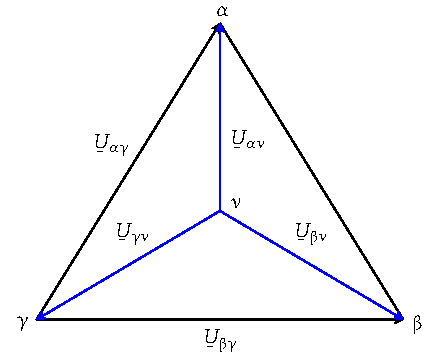
\includegraphics{Imatges/Cap-Fonaments-Potencia-Exemple.pdf}
    \end{minipage}
    \hfill
    \begin{minipage}[b][5.7cm][t]{3.8cm}
    \begin{align*}
        \cmplx{U}_{\alphaup\nuup} &= 220_{\angle 90\degree}\unit{V} \\[1ex]
        \cmplx{U}_{\betaup\nuup} &= 220_{\angle -30\degree}\unit{V} \\[1ex]
        \cmplx{U}_{\gammaup\nuup} &= 220_{\angle 210\degree}\unit{V} \\[1ex]
        \cmplx{U}_{\alphaup\gammaup} &= \sqrt{3}\cdot220_{\angle 60\degree}\unit{V} \\[1ex]
        \cmplx{U}_{\betaup\gammaup} &= \sqrt{3}\cdot220_{\angle 0\degree}\unit{V}
    \end{align*}
    \end{minipage}
    \hfill{}

    Els corrents $\cmplx{I}_\alphaup$, $\cmplx{I}_\betaup$ i $\cmplx{I}_\gammaup$ que
    circulen  per les tres fases s\'{o}n:
    \begin{align*}
        \cmplx{I}_\alphaup &=\frac{\cmplx{U}_{\alphaup\nuup}}{\cmplx{Z}} =
        \frac{220_{\angle 90\degree}\unit{V}}{22_{\angle
    45\degree}\unit{\ohm}} =
        10_{\angle 45\degree}\unit{A}\\
        \cmplx{I}_\betaup &=\frac{\cmplx{U}_{\betaup\nuup}}{\cmplx{Z}} =
        \frac{220_{\angle -30\degree}\unit{V}}{22_{\angle
    45\degree}\unit{\ohm}} =
        10_{\angle -75\degree}\unit{A}\\
        \cmplx{I}_\gammaup &=\frac{\cmplx{U}_{\gammaup\nuup}}{\cmplx{Z}} =
        \frac{220_{\angle 210\degree}\unit{V}}{22_{\angle
    45\degree}\unit{\ohm} } =
        10_{\angle 165\degree}\unit{A}
    \end{align*}


    Per comen\c{c}ar,  utilitzarem l'equaci\'{o} \eqref{eq:s_3f_eq}, ja que tenim
    un sistema equilibrat tant pel que fa a les tensions com pel que fa a la c\`{a}rrega:
    \[
    \cmplx{S} = 3\,\cmplx{U}_{\alphaup\nuup} \,\cmplx{I}_\alphaup^* =
    3\cdot 220_{\angle 90\degree}\unit{V} \cdot
    10_{\angle -45\degree}\unit{A} = 6600_{\angle 45\degree}\unit{VA}
    \]

    A continuaci\'{o},  utilitzarem l'equaci\'{o} \eqref{eq:s_3f_3fils}, ja que tenim
    un sistema d'alimentaci\'{o} de 3 fils:
    \[
    \cmplx{S} = \cmplx{U}_{\alphaup\gammaup} \,\cmplx{I}_\alphaup^*
     +  \cmplx{U}_{\betaup\gammaup} \,\cmplx{I}_\betaup^* =
    \sqrt{3}\cdot220_{\angle 60\degree}\unit{V} \cdot
    10_{\angle -45\degree}\unit{A} + \sqrt{3}\cdot220_{\angle 0\degree}\unit{V}
    \cdot 10_{\angle 75\degree}\unit{A}  = 6600_{\angle 45\degree}\unit{VA}
    \]

     Finalment,  utilitzarem l'equaci\'{o} \eqref{eq:s_3f}, ja que
     sempre \'{e}s aplicable:
     \[\begin{split}
     \cmplx{S} &=  \cmplx{U}_{\alphaup\nuup} \,\cmplx{I}_\alphaup^* +
     \cmplx{U}_{\betaup\nuup} \,\cmplx{I}_\betaup^* +  \cmplx{U}_{\gammaup\nuup}\,
     \cmplx{I}_\gammaup^* =\\
     &= 220_{\angle 90\degree}\unit{V}
     \cdot 10_{\angle -45\degree}\unit{A} + 220_{\angle
     -30\degree}\unit{V} \cdot 10_{\angle 75\degree}\unit{A}
     + 220_{\angle 210\degree}\unit{V} \cdot 10_{\angle
     -165\degree}\unit{A} =6600_{\angle 45\degree}\unit{VA}
     \end{split} \]

    Per acabar, veurem que tamb\'{e} es pot resoldre aquest exemple
    sense calcular les intensitats; si utilitzem a l'hora les
    equacions \eqref{eq:s_3f_eq} i \eqref{eq:s_mono1}, tenim:
    \[
    \cmplx{S} = 3\,\cmplx{U}_{\alphaup\nuup} \,\cmplx{I}_\alphaup^* = 3\,
    \frac{|\cmplx{U}_{\alphaup\nuup}|^2}{\cmplx{Z}^*} =
    3\cdot\frac{(220\unit{V})^2}{22_{\angle
    -45\degree}\unit{\ohm}} = 6600_{\angle 45\degree}\unit{VA}
    \]

    Com era d'esperar, el resultat obtingut en tots els casos
    \'{e}s id\`{e}ntic.
\end{exemple}

\subsection{Mesura de la pot\`{e}ncia}\index{pot\`{e}ncia complexa!mesura}

La pot\`{e}ncia activa es mesura amb uns aparells anomenats watt\'{\i}metres,
i la pot\`{e}ncia reactiva amb uns aparelles anomenats var\'{\i}metres.

Aquests aparells tenen dues bobines de mesura, una de voltim\`{e}trica,
la qual es connecta tal com es faria amb un volt\'{\i}metre, i una altra
d'amperim\`{e}trica, la qual es connecta tal com es faria amb un
amper\'{\i}metre; aix\'{\i} doncs, els watt\'{\i}metres i els var\'{\i}metres tenen
quatre terminals de connexi\'{o}.

La connexi\'{o} d'aquests aparells en un circuit donat, per tal de
mesurar correctament la pot\`{e}ncia, ve determinada pels dos terminals
anomenats hom\`{o}legs; un d'aquests terminals pertany a la bobina
voltim\`{e}trica i l'altre a l'amperim\`{e}trica. En els esquemes el\`{e}ctrics,
aquests dos terminals s'identifiquen mitjan\c{c}ant un punt. La connexi\'{o}
ha de fer-se de tal manera, que el corrent que va des de
l'alimentaci\'{o} cap a la c\`{a}rrega entri al watt\'{\i}metre pel terminal de
la bobina amperim\`{e}trica marcat amb el punt, i la tensi\'{o} corresponent
a aquest corrent, vagi del terminal de la bobina voltim\`{e}trica marcat
amb el punt, a l'altre terminal; el mateix \'{e}s aplicable al
var\'{\i}metre.

En la Figura \vref{pic:watt_var_mono} es pot veure la connexi\'{o} d'un
watt\'{\i}metre i d'un var\'{\i}metre en un circuit monof\`{a}sic.


\begin{figure}[h]
\centering
    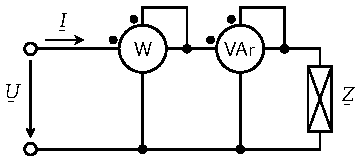
\includegraphics{Imatges/Cap-Fonaments-Mesura-Potencia-Monof.pdf}
\caption{Mesura de la pot\`{e}ncia en un circuit  monof\`{a}sic}
\label{pic:watt_var_mono}
\end{figure}

Les pot\`{e}ncies activa i reactiva s'obtenen de les mesures dels dos
aparells:
\begin{equation}
    P = \textsf{W} \qquad\qquad Q = \textsf{VAr}
\end{equation}

En la Figura \vref{pic:watt_var_4f} es pot veure la connexi\'{o} d'uns
watt\'{\i}metres i d'uns var\'{\i}metres en un circuit trif\`{a}sic de 4 fils,
equilibrat o desequilibrat.
\begin{figure}[htb]
\centering
    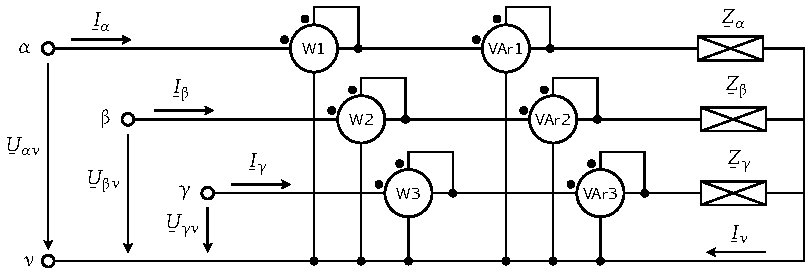
\includegraphics{Imatges/Cap-Fonaments-Mesura-Potencia-Trif-4f.pdf}
\caption{Mesura de la pot\`{e}ncia en un circuit  trif\`{a}sic de 4 fils}
\label{pic:watt_var_4f}
\end{figure}

Les pot\`{e}ncies activa i reactiva trif\`{a}siques s'obtenen de les mesures
dels sis aparells:
\begin{equation}
    P\ped{3F} = \textsf{W1} +  \textsf{W2} + \textsf{W3}
    \qquad\qquad Q\ped{3F} = \textsf{VAr1} +  \textsf{VAr2} + \textsf{VAr3}
\end{equation}

En la Figura \vref{pic:watt_var_3f} es pot veure la connexi\'{o} d'uns
watt\'{\i}metres i d'uns var\'{\i}metres en un circuit trif\`{a}sic de 3 fils,
equilibrat o desequilibrat.
\begin{figure}[htb]
\centering
    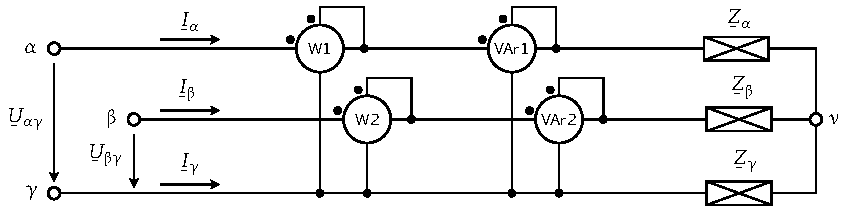
\includegraphics{Imatges/Cap-Fonaments-Mesura-Potencia-Trif-3f.pdf}
\caption{Mesura de la pot\`{e}ncia en un circuit  trif\`{a}sic de 3 fils}
\label{pic:watt_var_3f}
\end{figure}

Les pot\`{e}ncies activa i reactiva trif\`{a}siques s'obtenen de les mesures
dels quatre aparells:
\begin{equation}
    P\ped{3F} = \textsf{W1} +  \textsf{W2}
    \qquad\qquad Q\ped{3F} = \textsf{VAr1} +  \textsf{VAr2}
\end{equation}

\section{Valors mitj\`{a} i efica\c{c}, i factors d'amplitud, de forma i
d'arrissada}\label{sec:val_mitja_ef}

\subsection{Valor mitj\`{a}}\index{valor!mitj\`{a}}

El valor mitj\`{a} $V\ped{av}$ (de l'angl\`{e}s {"<}average{">}) d'una funci\'{o}
peri\`{o}dica en el temps $v(t)$, de freq\"{u}\`{e}ncia $f$, per\'{\i}ode $T$ i
velocitat angular $\omega$ ($f = 1/T$, $\omega=2\piup f = 2\piup\,/T$), es
defineix com:
\begin{equation}
    V\ped{av} = \frac{1}{T} \int_{t_0}^{t_0+T} v(t) \diff t =
    \frac{\omega}{2\piup} \int_{t_0}^{t_0+\frac{2\piup}{\omega}} v(t) \diff t\label{eq:vm_t}
\end{equation}

Si la funci\'{o} peri\`{o}dica $v(\alpha)$ est\`{a} definida en funci\'{o} de
l'angle $\alpha$, enlloc del temps $t$, a partir de la relaci\'{o}
$\alpha=\omega t$ ($\diff\alpha=\omega\diff t$), tenim:
\begin{equation}
    V\ped{av} = \frac{1}{2\piup} \int_{\alpha_0}^{\alpha_0+2\piup} v(\alpha) \diff \alpha
    \label{eq:vm_alfa}
\end{equation}

\subsection{Valor efica\c{c}}\index{valor!efica\c{c}}
\index{root mean square@\guillemotleft root mean
square\guillemotright}\index{rms}

El valor efica\c{c}  $V$ (tamb\'{e} anomenat valor rms, de l'angl\`{e}s {"<}root
mean square{">}) d'una funci\'{o} peri\`{o}dica en el temps $v(t)$, de
freq\"{u}\`{e}ncia $f$, per\'{\i}ode $T$ i velocitat angular $\omega$ ($f = 1/T$,
$\omega=2\piup f = 2\piup\,/T$), es defineix com:
\begin{equation}
    V = \sqrt{\frac{1}{T} \int_{t_0}^{t_0+T} [v(t)]^2 \diff
    t} = \sqrt{\frac{\omega}{2\piup} \int_{t_0}^{t_0+\frac{2\piup}{\omega}}
     [v(t)]^2 \diff t}
\end{equation}

Si la funci\'{o} peri\`{o}dica $v(\alpha)$ est\`{a} definida en funci\'{o} de
l'angle $\alpha$, enlloc del temps $t$, a partir de la relaci\'{o}
$\alpha=\omega t$ ($\diff\alpha=\omega\diff t$), tenim:
\begin{equation}
    V = \sqrt{\frac{1}{2\piup} \int_{\alpha_0}^{\alpha_0+2\piup}
     [v(\alpha)]^2 \diff \alpha}
\end{equation}

\subsection{Factor d'amplitud o de cresta}\index{factor!d'amplitud}
\index{factor!de cresta}\index{fa@$f\ped{a}$}

El factor d'amplitud $f\ped{a}$ relaciona el valor m\`{a}xim o de cresta
$\hat{V}$ d'una funci\'{o} peri\`{o}dica, amb el seu valor efica\c{c} $V$:
\begin{equation}
    f\ped{a} = \frac{\hat{V}}{V}
\end{equation}

\subsection{Factor de forma}\index{factor!de forma}\index{ff@$f\ped{f}$}

El factor de forma $f\ped{f}$ relaciona els valors mitj\`{a} $V\ped{av}$
i efica\c{c} $V$ d'una funci\'{o} peri\`{o}dica:
\begin{equation}
    f\ped{f} = \frac{V}{V\ped{av}}
\end{equation}

\subsection{Factor d'arrissada}\index{factor!d'arrissada}\index{r}
\index{ripple@\guillemotleft ripple\guillemotright}

El factor d'arrissada $r$ (de l'angl\`{e}s {"<}ripple{">}) relaciona els
valors mitj\`{a} $V\ped{av}$ i efica\c{c} $V$ d'una funci\'{o} peri\`{o}dica.

Aquest factor s'utilitza usualment per definir la qualitat d'una
tensi\'{o} continua, rectificada a partir d'una tensi\'{o} alterna. Com m\'{e}s
plana sigui aquesta tensi\'{o} cont\'{\i}nua m\'{e}s baix ser\`{a} el seu factor
d'arrissada:
\begin{equation}
    r = \sqrt{\left(\frac{V}{V\ped{av}}\right)^2-1} = \sqrt{f\ped{f}^2-1}
\end{equation}

\begin{exemple}
Es tracta de calcular els factors d'amplitud, de forma i d'arrissada
de la tensi\'{o}  que s'obt\'{e}, a partir d'una tensi\'{o} sinuso\"{\i}dal
$u(t) = \hat{U} \sin\omega t$, amb un rectificador de mitja ona i
amb un rectificador d'ona completa.

En el cas del rectificador de mitja ona, la tensi\'{o} que s'obt\'{e} ve
definida per:
\[
u(t) = \begin{cases} \hat{U} \sin\omega t, & 0 < \omega t < \piup\\
       0, & \piup \leq \omega t \leq 2\piup \end{cases}
\]

Calculem en primer lloc el valor mitj\`{a}:
\[
U\ped{av} = \frac{\omega}{2\piup} \left( \int_0^\frac{\piup}{\omega}
\hat{U} \sin\omega t \diff t +
\int_\frac{\piup}{\omega}^\frac{2\piup}{\omega} 0 \diff t \right) = -
\left. \frac{\hat{U} \cos\omega t}{2\piup}
\right|_0^\frac{\piup}{\omega} = \frac{\hat{U}}{\piup}
\]

Calculem a continuaci\'{o} el valor efica\c{c}:
\[
U = \sqrt{\frac{\omega}{2\piup} \left( \int_0^\frac{\piup}{\omega}
\hat{U}^2 \sin^2\omega t \diff t +
\int_\frac{\piup}{\omega}^\frac{2\piup}{\omega} 0 \diff t \right)} =
  \sqrt{\left.\frac{\omega \hat{U}^2}{2\piup}\left( \frac{t}{2} -
\frac{\sin (2\omega t)}{4\omega}
\right)\right|_0^\frac{\piup}{\omega}} = \frac{\hat{U}}{2}
\]

Els factors d'amplitud, de forma i d'arrissada s\'{o}n:
\begin{align*}
    f\ped{a} &= \frac{\hat{U}}{\hat{U}/2} = 2 \\[0.5ex]
    f\ped{f} &= \frac{\hat{U}/2}{\hat{U}/\piup} =\frac{\piup}{2} =
    1{,}57 \\[0.5ex]
    r &= \sqrt{\left(\frac{\hat{U}/2}{\hat{U}/\piup}\right)^2-1} =
\sqrt{\frac{\piup^2}{4}-1} = 1{,}21
\end{align*}


En el cas del rectificador d'ona completa, la tensi\'{o} que s'obt\'{e} ve
definida per:
\[
u(t) = \begin{cases} \phantom{-}\hat{U} \sin\omega t, & 0 < \omega t < \piup\\
       -\hat{U} \sin\omega t, & \piup \leq \omega t \leq 2\piup \end{cases}
\]

En aquest cas, l'ona de tensi\'{o} entre $\piup$ i $2\piup$ \'{e}s una repetici\'{o}
exacta de l'ona de tensi\'{o} entre 0 i $\piup$, per tant, \'{u}nicament
caldr\`{a} considerar-ne la primera meitat (entre 0 i $\piup$), tenint en
compte que el per\'{\i}ode ser\`{a} $\piup\,/\omega$.

 Calculem en primer lloc el valor mitj\`{a}:
\[
U\ped{av} = \frac{\omega}{\piup} \int_0^\frac{\piup}{\omega} \hat{U}
\sin\omega t \diff t  = - \left. \frac{\hat{U} \cos\omega t}{\piup}
\right|_0^\frac{\piup}{\omega} = \frac{2 \hat{U}}{\piup}
\]

Calculem a continuaci\'{o} el valor efica\c{c}:
\[
U = \sqrt{\frac{\omega}{\piup} \int_0^\frac{\piup}{\omega} \hat{U}^2
\sin^2\omega t \diff t } =   \sqrt{\left.\frac{\omega
\hat{U}^2}{\piup}\left( \frac{t}{2} - \frac{\sin (2\omega t)}{4\omega}
\right)\right|_0^\frac{\piup}{\omega}}  = \frac{\hat{U}}{\sqrt{2}}
\]

Els factors d'amplitud, de forma i d'arrissada s\'{o}n:
\begin{align*}
    f\ped{a} &= \frac{\hat{U}}{\hat{U}/\sqrt{2}} = \sqrt{2} \\[0.5ex]
    f\ped{f} &= \frac{\hat{U}/\sqrt{2}}{2 \hat{U}/\piup} =\frac{\piup}{2\sqrt{2}} =
    1{,}11 \\[0.5ex]
r &= \sqrt{\left(\frac{\hat{U}/\sqrt{2}}{2 \hat{U}/\piup}\right)^2-1}
= \sqrt{\frac{\piup^2}{8}-1} = 0{,}48
\end{align*}

\end{exemple}


\section{Circuits divisors de tensi\'{o} i divisors de corrent}\label{sec:div_tens_corr}

Un circuit divisor de tensi\'{o} est\`{a} format per un conjunt
d'imped\`{a}ncies en s\`{e}rie, i el que es pret\'{e}n \'{e}s calcular la caiguda de
tensi\'{o} en cada imped\`{a}ncia, en funci\'{o} de la caiguda de tensi\'{o} total.

Un circuit divisor de corrent, en canvi, est\`{a} format per un conjunt
d'imped\`{a}ncies en para{\l.l}el, i el que es pret\'{e}n \'{e}s calcular el
corrent que circula per cada imped\`{a}ncia, en funci\'{o} del corrent
total.

\subsection{Circuits divisors de tensi\'{o}}\index{circuits divisors!de
tensi\'{o}}

En la Figura \vref{pic:div_tensio} es pot veure un circuit divisor
de tensi\'{o}, pel qual es vol calcular la caiguda de tensi\'{o}
$\cmplx{U}_i$ en la imped\`{a}ncia $\cmplx{Z}_i$, a partir de la caiguda
de tensi\'{o} total $\cmplx{U}\ped{total}$.
\begin{figure}[htb]
\centering
    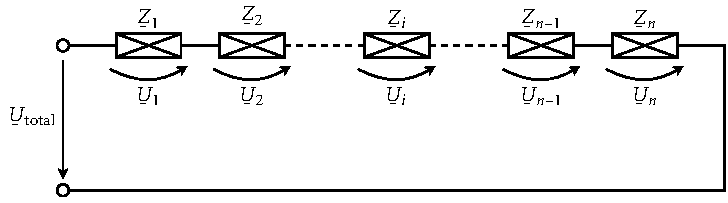
\includegraphics{Imatges/Cap-Fonaments-Divisor-Tensio.pdf}
\caption{Circuit divisor de tensi\'{o}} \label{pic:div_tensio}
\end{figure}

La imped\`{a}ncia total $\cmplx{Z}\ped{total}$ del circuit val:
\begin{equation}
    \cmplx{Z}\ped{total} = \sum_{i=1}^n \cmplx{Z}_i
\end{equation}

Utilitzant aquest valor, la tensi\'{o} $\cmplx{U}_i$ val:
\begin{equation}
    \cmplx{U}_i = \frac{\cmplx{Z}_i}{\cmplx{Z}\ped{total}}\,\cmplx{U}\ped{total}
\end{equation}

\subsection{Circuits divisors de corrent}\index{circuits divisors!de
corrent}

En la Figura \vref{pic:div_corrent} es pot veure un circuit divisor
de corrent, pel qual es vol calcular el corrent $\cmplx{I}_i$ que
circula per la imped\`{a}ncia $\cmplx{Z}_i$, a partir del corrent total
$\cmplx{I}\ped{total}$.
\begin{figure}[htb]
\centering
    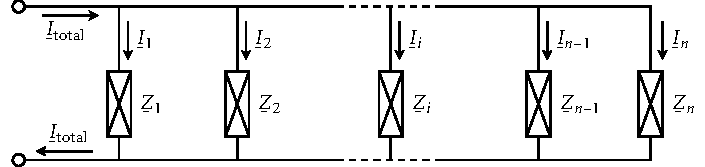
\includegraphics{Imatges/Cap-Fonaments-Divisor-Corrent.pdf}
\caption{Circuit divisor de corrent} \label{pic:div_corrent}
\end{figure}

La imped\`{a}ncia total $\cmplx{Z}\ped{total}$ del circuit val:
\begin{equation}
    \cmplx{Z}\ped{total} = \frac{1}{\displaystyle\sum_{i=1}^n \frac{1}{\cmplx{Z}_i}}
\end{equation}

Utilitzant aquest valor, el corrent $\cmplx{I}_i$ val:
\begin{equation}
    \cmplx{I}_i = \frac{\cmplx{Z}\ped{total}}{\cmplx{Z}_i}\,\cmplx{I}\ped{total}
\end{equation}



\section{C\`{a}lculs en p.u.} \label{sec:seccio_pu} \index{p.u.}

Les magnituds expressades en p.u.\ (per unitat) s\'{o}n \'{u}tils quan es treballa
amb xarxes de corrent altern on hi ha transformadors, i per tant m\'{e}s d'un nivell de tensi\'{o}.

\subsection{M\`{e}tode de c\`{a}lcul} \index{p.u.!m\`{e}tode de c\`{a}lcul}

\index{p.u.!magnituds base fonamentals} El primer pas consisteix a
escollir unes magnituds base. Les magnituds base fonamentals s\'{o}n la
pot\`{e}ncia i la tensi\'{o}; s'escull una pot\`{e}ncia base $S\ped{B}$ per a
tota la xarxa, i tantes tensions base com nivells de tensi\'{o}
diferents tingui la xarxa $U_{\text{B}_1}, U_{\text{B}_2}, \ldots,
U_{\text{B}_n}$:
\begin{equation}
   \text{Magnituds base fonamentals}\;\left\{
\begin{array}{l}
   S\ped{B} \\
   U_{\text{B}_1}, U_{\text{B}_2}, \ldots, U_{\text{B}_n}
\end{array}
\right.
\end{equation}

Normalment s'escull com a tensions base les tensions nominals dels transformadors de la
xarxa, i com a pot\`{e}ncia base la potencia nominal d'un del transformadors o generadors de la xarxa; tamb\'{e} \'{e}s usual utilitzar com a pot\`{e}ncia base el valor 100\unit{MVA}.

En el cas de circuits monof\`{a}sics, les tensions base s\'{o}n les tensions monof\`{a}siques, o fase--neutre $U\ped{FN}$, i la pot\`{e}ncia base \'{e}s la potencia monof\`{a}sica $S\ped{1F}$. En el cas de circuits trif\`{a}sics, podem escollir com a tensions base les tensions fase--neutre $U\ped{FN}$ i com a pot\`{e}ncia base la pot\`{e}ncia  monof\`{a}sica $S\ped{1F}$, o b\'{e} podem escollir com a tensions base les tensions fase--fase $U\ped{FF}$ i com a pot\`{e}ncia base la potencia trif\`{a}sica $S\ped{3F}$.

\index{p.u.!magnituds base}A partir de la pot\`{e}ncia base i de les tensions base es
defineixen els corrents base $I_{\text{B}_i}$, les imped\`{a}ncies base $Z_{\text{B}_i}$ i les
admit\`{a}ncies base $Y_{\text{B}_i}$. Segons que s'utilitzin les tensions i pot\`{e}ncies monof\`{a}siques o trif\`{a}siques com a magnituds base, tenim:
\begin{equation}
\begin{array}{c}  S\ped{B}=S\ped{1F} \\ U_{\text{B}_i} = U_{\text{FN}_i} \\ (i=1,\ldots,n) \end{array}
\left\{
\begin{array}{lll}
   I_{\text{B}_i} &= &\dfrac{S\ped{B}}{U_{\text{B}_i}} \\[2.5ex]
   Z_{\text{B}_i} &= &\dfrac{U_{\text{B}_i}^2}{S\ped{B}} \\[2.5ex]
   Y_{\text{B}_i} &= &\dfrac{S\ped{B}}{U_{\text{B}_i}^2}
\end{array}
\right.
\qquad\qquad
\begin{array}{c} S\ped{B}=S\ped{3F} \\ U_{\text{B}_i} = U_{\text{FF}_i} \\ (i=1,\ldots,n) \end{array}
\left\{
\begin{array}{llc}
   I_{\text{B}_i} &= &\dfrac{S\ped{B}}{\sqrt{3} U_{\text{B}_i}} \\[2.5ex]
   Z_{\text{B}_i} &= &\dfrac{U_{\text{B}_i}^2}{S\ped{B}} \\[2.5ex]
   Y_{\text{B}_i} &= &\dfrac{S\ped{B}}{U_{\text{B}_i}^2}
\end{array}
\right.
\label{eq:bases_pu}
\end{equation}

Les magnituds expressades en p.u.\ (escrites usualment en min\'{u}scules) s'obtenen
dividint les magnituds reals (escrites usualment en maj\'{u}scules) pels valors base corresponents:
\begin{equation}
   \cmplx{s} = \frac{\cmplx{S}}{S\ped{B}} \qquad \cmplx{u} = \frac{\cmplx{U}}{U\ped{B}} \qquad \cmplx{i} = \frac{\cmplx{I}}{I\ped{B}} \qquad \cmplx{z} = \frac{\cmplx{Z}}{Z\ped{B}} \qquad \cmplx{y} = \frac{\cmplx{Y}}{Y\ped{B}}
\end{equation}

Quan es tracta de resoldre circuits trif\`{a}sics equilibrats fem servir sempre els circuits equivalents per fase, i podem escollir aleshores com a valors base per a la pot\`{e}ncia i la tensi\'{o}, la pot\`{e}ncia monof\`{a}sica $S\ped{1F}$ i la tensi\'{o} fase--neutre $U\ped{FN}$ respectivament, o la pot\`{e}ncia trif\`{a}sica $S\ped{3F}$ i la tensi\'{o} fase--fase $U\ped{FF}$ respectivament; quan fem la reducci\'{o} de valors reals a valors en p.u., hem de ser conseq\"{u}ents i utilitzar sempre les pot\`{e}ncies monof\`{a}siques i les tensions fase-neutre en el primer cas, i les pot\`{e}ncies trif\`{a}siques i les tensions fase-fase en el segon cas. Donat que es verifica $S\ped{3F}=3 S\ped{1F}$ i $U\ped{FF}=\sqrt{3}U\ped{FN}$, els valors  del corrent base $I\ped{B}$, de la imped\`{a}ncia base $Z\ped{B}$ i  de l'admit\`{a}ncia base $Y\ped{B}$ s\'{o}n els mateixos, tan si utilitzem $S\ped{B}=S\ped{1F}$ i $U\ped{B}=U\ped{FN}$, con si utilitzem $S\ped{B}=S\ped{3F}$ i $U\ped{B}=U\ped{FF}$. En ambd\'{o}s casos $I\ped{B}$ i $\cmplx{I}$ s\'{o}n corrents fase--neutre, $Z\ped{B}$ i $\cmplx{Z}$ s\'{o}n imped\`{a}ncies fase--neutre i $Y\ped{B}$ i $\cmplx{Y}$ s\'{o}n admit\`{a}ncies fase--neutre; si tenim c\`{a}rregues connectades en triangle, cal transformar-les en c\`{a}rregues equivalents connectades en estrella per tal de poder aplicar aquest m\`{e}tode (vegeu la secci\'{o} \ref{secc:d_y}).

El pas seg\"{u}ent consisteix a representar el circuit equivalent en
p.u.\ i resoldre'l; en el cas de circuits trif\`{a}sics, i com a conseq\"{u}\`{e}ncia del proc\'{e}s utilitzat, el circuit equivalent en p.u.\ \'{e}s un circuit monof\`{a}sic i com a tal l'hem de resoldre, \'{e}s a dir, sense la intervenci\'{o} del factor $\sqrt{3}$.

Un cop resolt el circuit, es multipliquen les magnituds obtingudes en p.u.\ pels
seus valors base respectius, per tal d'obtenir les magnituds reals:
\begin{equation}
   \cmplx{S} = \cmplx{s} S\ped{B} \qquad \cmplx{U} = \cmplx{u} U\ped{B} \qquad \cmplx{I} = \cmplx{i} I\ped{B} \qquad \cmplx{Z} = \cmplx{z} Z\ped{B} \qquad \cmplx{Y} = \cmplx{y} Y\ped{B}
\end{equation}

\subsection{Canvi de base}\label{sec:canvi-base} \index{p.u.!canvi de base}

Normalment les imped\`{a}ncies de transformadors (imped\`{a}ncia de curt circuit) o de generadors (imped\`{a}ncia sincr\`{o}nica, transit\`{o}ria, etc.) estan referides a les magnituds nominals de la m\`{a}quina en q\"{u}esti\'{o}. Si les magnituds base escollides coincideixen amb les nominals de la m\`{a}quina,
la imped\`{a}ncia de la m\`{a}quina en q\"{u}esti\'{o} estar\`{a} expressada ja directament en p.u.; en canvi si les magnituds base s\'{o}n diferents de les nominals de la m\`{a}quina, caldr\`{a} fer un canvi de base per tal de referir la imped\`{a}ncia de la m\`{a}quina a les magnituds base escollides.

De forma gen\`{e}rica, si $\cmplx{z}$ \'{e}s una imped\`{a}ncia referida a la base $U\ped{B}$ i $S\ped{B}$, podem obtenir la imped\`{a}ncia $\cmplx{z}'$ referida a la base $U_{\text{B}'}$ i $S_{\text{B}'}$, mitjan\c{c}ant el canvi:
\begin{equation}
   \cmplx{z}' = \cmplx{z} \; \frac{Z\ped{B}}{Z\ped{B}'} = \cmplx{z} \; \frac{U\ped{B}^2}{S\ped{B}} \; \frac{S_{\text{B}'}}{U_{\text{B}'}^2}
\end{equation}

\begin{exemple}

Es tracte de calcular el corrent de curt circuit trif\`{a}sic en el punt F de la xarxa seg\"{u}ent, suposant
que el sistema est\`{a} treballant en buit.
\begin{figure}[htb]
\vspace{3mm} \centering
    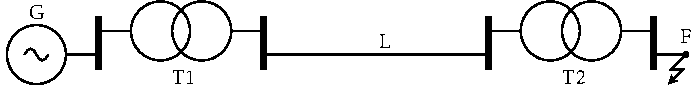
\includegraphics{Imatges/Cap-Fonaments-pu-Circuit1.pdf}
\end{figure}

Les dades del generador G, del transformador T1, de la l\'{\i}nia L i del transformador T2 s\'{o}n:
\begin{align*}
   S\ped{G} &= 60\unit{MVA} & S\ped{T1} &= 40\unit{MVA} & l\ped{L} &= 22\unit{km} & S\ped{T2} &= 12\unit{MVA} \\
   U\ped{G} &= 10{,}5\unit{kV} & m\ped{T1} &= 10{,}5\unit{kV}\!:\!63\unit{kV} & U\ped{L} &= 60\unit{kV} & m\ped{T2} &= 60\unit{kV}\!:\!10{,}5\unit{kV} \\
   X''\ped{G} &= 12\unit{\%} & X\ped{T1} &= 10\unit{\%} & X\ped{L} &= 0,4\unit{\ohm/km} & X\ped{T2} &= 8\unit{\%}
\end{align*}

Escollim en primer lloc les seg\"{u}ents magnituds base: $S\ped{B} = 60\unit{MVA}$ i $U\ped{B}
= 10{,}5\unit{kV} / 63\unit{kV} / 10{,}5\unit{kV}$.

Calculem a continuaci\'{o} els valors en p.u.\ dels diferents elements de la xarxa:

\textbf{Generador}. En coincidir les magnituds base amb les nominals del generador tenim
 directament:
\[
x''\ped{G} = 0{,}12\unit{p.u.}
\]

\textbf{Transformador 1}. La relaci\'{o} de transformaci\'{o} i la react\`{a}ncia s\'{o}n respectivament:
\[
m\ped{T1} = \frac{10{,}5\unit{kV}}{10{,}5\unit{kV}} :
\frac{63\unit{kV}}{63\unit{kV}} = 1\!:\!1 \qquad\qquad x\ped{T1} =
0{,}10 \cdot \frac{(63\unit{kV})^2}{40\unit{MVA}} \cdot
\frac{60\unit{MVA}}{(63\unit{kV})^2}  = 0{,}15\unit{p.u.}
\]

\textbf{L\'{\i}nia}. La react\`{a}ncia \'{e}s:
\[x\ped{L} = \frac{0{,}4\unit{\ohm/km} \cdot 22\unit{km}} {(63\unit{kV})^2/60\unit{MVA}}  = 0{,}1330\unit{p.u.}
\]

\textbf{Transformador 2}. La relaci\'{o} de transformaci\'{o} i la react\`{a}ncia s\'{o}n respectivament:
\[
m\ped{T2} = \frac{60\unit{kV}}{63\unit{kV}} :
\frac{10{,}5\unit{kV}}{10{,}5\unit{kV}} = 0{,}9524\!:\!1 \qquad\qquad
x\ped{T2} = 0{,}08 \cdot \frac{(10{,}5\unit{kV})^2}{12\unit{MVA}}
\cdot \frac{60\unit{MVA}}{(10{,}5\unit{kV})^2}  = 0{,}4\unit{p.u.}
\]

\textbf{Tensi\'{o} en el punt F}. La tensi\'{o} abans del curt circuit \'{e}s la mateixa que la del generador G, elevada pel transformador T1 i redu\"{\i}da despr\'{e}s pel transformador T2:
\[
\cmplx{u}\ped{F} = \frac{10{,}5\unit{kV} \cdot
\dfrac{63\unit{kV}}{10{,}5\unit{kV}} \cdot
\dfrac{10{,}5\unit{kV}}{60\unit{kV}}}{10{,}5\unit{kV}} =
1{,}05\unit{p.u.}
\]

A partir d'aquests valors calculats, tenim el seg\"{u}ent circuit equivalent en p.u.\ durant el
curt circuit en el punt F:
\begin{figure}[h]
\vspace{3mm} \centering
   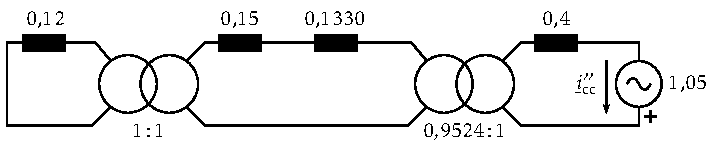
\includegraphics{Imatges/Cap-Fonaments-pu-Circuit2.pdf}
\end{figure}


El corrent de curt circuit buscat val:
\[
|\cmplx{i}''\ped{cc}| = \left| \frac{1{,}05}{\ju \left( 0{,}4 + \frac{0{,}15 + 0{,}1330}{0{,}9524^2} + \frac{0{,}12}{0{,}9524^2 \cdot 1^2} \right)} \right| = 1{,}2436\unit{p.u.} \qquad |\cmplx{I}''\ped{cc}| = 1{,}2436\cdot\frac{60\unit{MVA}}{\sqrt{3}\cdot 10{,}5\unit{kV}} = 4{,}1\unit{kA}
\]

 A l'hora de calcular el corrent de curt circuit utilitzant el circuit equivalent en p.u.,
 s'observa que el transformador T1 \'{e}s com si hagu\'{e}s desaparegut,
 aix\`{o} \'{e}s aix\'{\i}, ja que la seva relaci\'{o} de transformaci\'{o} ha esdevingut
 $1\!:\!1$, en coincidir les tensions base amb les seves tensions nominals;
 no passa el mateix amb el transformador T2, ja que no es compleix
 la coincid\`{e}ncia entre les seves tensions nominals i les tensions
 base. No obstant, at\`{e}s que l'elecci\'{o} de les tensions base \'{e}s
 arbitr\`{a}ria, si en lloc de 10,5\unit{kV} com a tercera tensi\'{o} base,
 escollim
 $\frac{63\unit{kV}}{60\unit{kV} / 10{,}5\unit{kV}}=11{,}025\unit{kV}$,
 tindrem:
\begin{align*}
   m\ped{T2} &= \frac{60\unit{kV}}{63\unit{kV}} : \frac{10{,}5\unit{kV}}{11{,}025\unit{kV}}
   = 0{,}9524\!:\!0{,}9524 = 1\!:\!1 \\
   x\ped{T2} &= 0{,}08 \cdot \frac{(10{,}5\unit{kV})^2}{12\unit{MVA}} \cdot
   \frac{60\unit{MVA}}{(11{,}025\unit{kV})^2}  = 0{,}3628\unit{p.u.}\\
   \cmplx{u}\ped{F} &= \frac{10{,}5\unit{kV} \cdot \dfrac{63\unit{kV}}{10{,}5\unit{kV}} \cdot
   \dfrac{10{,}5\unit{kV}}{60\unit{kV}}}{11{,}025\unit{kV}} = 1\unit{p.u.}
\end{align*}

Utilitzant aquests nous valors, podem prescindir totalment dels dos
transformadors, i calcular el corrent de curt circuit utilitzant
l'expressi\'{o} seg\"{u}ent:
\[
|\cmplx{i}''\ped{cc}| = \left| \frac{1}{\ju ( 0{,}3628 + 0{,}15 +
0{,}1330 + 0{,}12 )} \right| = 1{,}3058\unit{p.u.} \qquad
|\cmplx{I}''\ped{cc}| =
1{,}3058\cdot\frac{60\unit{MVA}}{\sqrt{3}\cdot 11{,}025\unit{kV}} =
4{,}1\unit{kA}
\]

Evidentment, el valor final \'{e}s el mateix independentment de quines
siguin les tensions base escollides.
\end{exemple}

\subsection{Valors base per a branques que treballen a diferent tensi\'{o}, amb acoblament magn\`{e}tic}\index{p.u.!acoblament magn\`{e}tic}

En la figura \vref{pic:pu_zm} hi ha representades dues branques acoblades magn\`{e}ticament; es fa el sup\`{o}sit addicional que les tensions de treball de les dues branques s\'{o}n diferents.
\begin{figure}[h]
\centering
    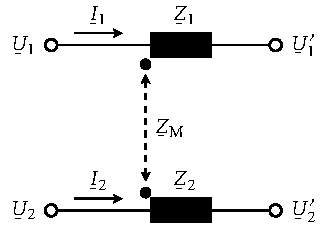
\includegraphics{Imatges/Cap-Fonaments-pu-ZM.pdf}
    \caption{Valors base en un acoblament magn\`{e}tic} \label{pic:pu_zm}
\end{figure}

Les equacions que relacionen els corrents i les tensions d'aquest circuit s\'{o}n:
\begin{subequations}
\begin{align}
    \cmplx{U}_1 - \cmplx{U}'_1 &= \cmplx{Z}_1 \cmplx{I}_1 + \cmplx{Z}\ped{M} \cmplx{I}_2   \\[2mm]
    \cmplx{U}_2 - \cmplx{U}'_2 &= \cmplx{Z}_2 \cmplx{I}_2 + \cmplx{Z}\ped{M} \cmplx{I}_1
\end{align}
\end{subequations}

Si volem convertir aquestes magnituds a valors en p.u., hem d'escollir  una potencia base $S\ped{B}$ i dues tensions base, una  per a cada branca, $U_{\text{B}_1}$ i  $U_{\text{B}_2}$, i a partir de les equacions \eqref{eq:bases_pu} obtenir els corrents, imped\`{a}ncies i admit\`{a}ncies base per a cada branca.

De la mateixa manera que s'ha dit en els apartats anteriors, en el cas de circuits trif\`{a}sics, podem escollir com a tensions base les tensions fase--neutre $U\ped{FN}$ i com a pot\`{e}ncia base la pot\`{e}ncia  monof\`{a}sica $S\ped{1F}$, o b\'{e} podem escollir com a tensions base les tensions fase--fase $U\ped{FF}$ i com a pot\`{e}ncia base la potencia trif\`{a}sica $S\ped{3F}$.


Per tal de calcular la imped\`{a}ncia base $Z_{\text{B}_\text{M}}$ per convertir $\cmplx{Z}\ped{M}$ en un valor en p.u., no podem utilitzar les equacions \eqref{eq:bases_pu}, ja que cadascun dels dos extrems de l'acoblament magn\`{e}tic est\`{a} a una tensi\'{o} diferent; en aquest cas, cal utilitzar l'equaci\'{o} que es por trobar en \cite{TLE}:
\begin{equation}
    Z_{\text{B}_\text{M}} = \frac{U_{\text{B}_1} U_{\text{B}_2}} {S\ped{B}}
\end{equation}

El valor en p.u.\ $\cmplx{z}\ped{M}$ corresponent a $\cmplx{Z}\ped{M}$ s'obt\'{e} de la manera usual:
\begin{equation}
    \cmplx{z}\ped{M} = \frac{\cmplx{Z}\ped{M}}{Z_{\text{B}_\text{M}}}
\end{equation}


\subsection{Valors base per a branques que treballen a diferent tensi\'{o}, amb acoblament capacitiu}\index{p.u.!acoblament capacitiu}

En la figura \vref{pic:pu_ym} hi ha representades dues branques acoblades capacitivament; es fa el sup\`{o}sit addicional que les tensions de treball de les dues branques s\'{o}n diferents.
\begin{figure}[!h]
\centering
    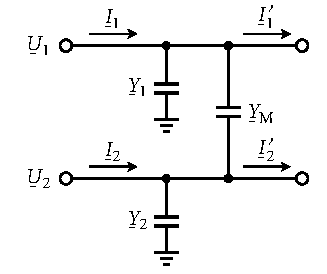
\includegraphics{Imatges/Cap-Fonaments-pu-YM.pdf}
    \caption{Valors base en un acoblament capacitiu} \label{pic:pu_ym}
\end{figure}

Les equacions que relacionen els corrents i les tensions d'aquest circuit s\'{o}n:
\begin{subequations}
\begin{align}
    \cmplx{I}_1  &= \cmplx{Y}_1 \cmplx{U}_1 +  \cmplx{Y}\ped{M}(\cmplx{U}_1-\cmplx{U}_2)  + \cmplx{I}'_1   \\[2mm]
    \cmplx{I}_2  &= \cmplx{Y}_2 \cmplx{U}_2 +  \cmplx{Y}\ped{M}(\cmplx{U}_2-\cmplx{U}_1)  + \cmplx{I}'_2
\end{align}
\end{subequations}

Si volem convertir aquestes magnituds a valors en p.u., hem d'escollir  una potencia base $S\ped{B}$ i dues tensions base, una  per a cada branca, $U_{\text{B}_1}$ i  $U_{\text{B}_2}$, i a partir de les equacions \eqref{eq:bases_pu} obtenir els corrents, imped\`{a}ncies i admit\`{a}ncies base per a cada branca.

De la mateixa manera que s'ha dit en els apartats anteriors, en el cas de circuits trif\`{a}sics, podem escollir com a tensions base les tensions fase--neutre $U\ped{FN}$ i com a pot\`{e}ncia base la pot\`{e}ncia  monof\`{a}sica $S\ped{1F}$, o b\'{e} podem escollir com a tensions base les tensions fase--fase $U\ped{FF}$ i com a pot\`{e}ncia base la potencia trif\`{a}sica $S\ped{3F}$.


Per tal de  calcular l'admit\`{a}ncia base $Y_{\text{B}_\text{M}}$ per convertir $\cmplx{Y}\ped{M}$ en un valor en p.u., no podem utilitzar les equacions \eqref{eq:bases_pu}, ja que cadascun dels dos extrems de l'acoblament capacitiu est\`{a} a una tensi\'{o} diferent; en aquest cas, cal utilitzar l'equaci\'{o} que es por trobar en \cite{TLE}:
\begin{equation}
    Y_{\text{B}_\text{M}} = \frac{S\ped{B}}{U_{\text{B}_1} U_{\text{B}_2}}
\end{equation}

El valor en p.u.\ $\cmplx{y}\ped{M}$ corresponent a $\cmplx{Y}\ped{M}$ s'obt\'{e} de la manera usual:
\begin{equation}
    \cmplx{y}\ped{M} = \frac{\cmplx{Y}\ped{M}}{Y_{\text{B}_\text{M}}}
\end{equation}
